\documentclass[11pt, letterpaper]{article}
\usepackage[utf8]{inputenc} %Paquete de Codificación
\usepackage[spanish]{babel} %Paquete de idioma
\usepackage{enumitem}       %Paquete para listas
\usepackage{graphicx}       %Paquete para imagenas
\usepackage{amsmath}        %Paquete para matematicas
\usepackage{lipsum}         %Paquete para texto aleatorio
\usepackage{hyperref}
\usepackage{listings}
\usepackage{subfig}
\graphicspath{ {img/} }  %Path para carpeta imagenes



\begin{document}

\begin{titlepage}
	\centering
	{\bfseries\LARGE Universidad de Alicante\par}
	\vspace{1cm}
	{\scshape\Large Escuela Politecnica Superior\par}
	\vspace{3cm}
	{\scshape\Huge Entregable 2\par}
	\vspace{3cm}
	\vfill
	{\Large Autor: \par}
	{\Large David Carbonell Pastor \par}
	\vfill
	{\Large 2022\par}
\end{titlepage}

\tableofcontents

\pagebreak

\section{Uso de la plataforma IoT Ubidots}
\subsection{Evidencias del trabajo realizado}
Se ha utilizado la plataforma IoT Ubidots a través de Node-Red como se puede ver en la figura \ref{fig:ubidots_nodered}
de esta manera se simplifica el apartado de la programación ya que de otra manera se ha de realizar mediante codigo python para
lo que pretendemos implementar.
\begin{figure}[h]
	\centering
	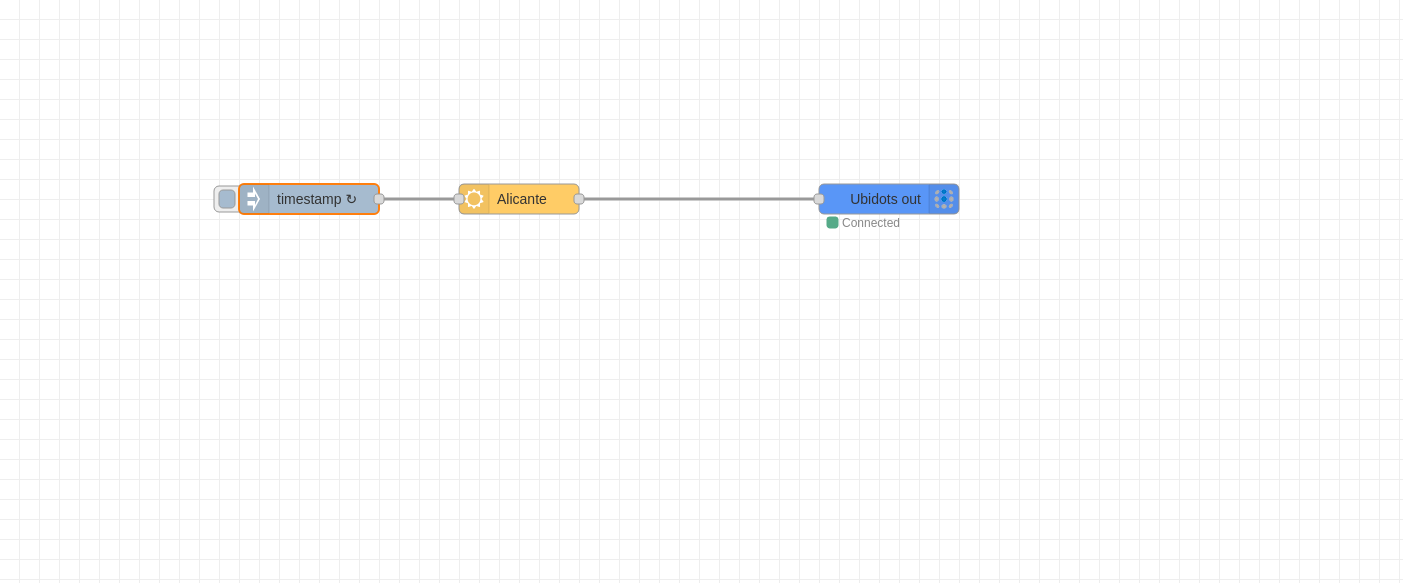
\includegraphics[width=\textwidth]{ubidots_nodered.png}
	\caption{Conexion de ubidots con nodered}
	\label{fig:ubidots_nodered}
\end{figure}

Enviamos la información del nodo de openweather al nodo de ubidots
en la pagina de ubidots en el apartado devices nos aparecen los parametros
que nos proporciona en formato json de una manera mas visual donde podemos ver los
distintos datos que tenemos.\\


Con los datos proporcionados por el nodo de openweather se ha realizado un dashboard simple \ref{fig:dashboard_ejemplo}
el cual presenta una menor complejidad y mayores funcionalidades que los dashboard creados con node-red
en el anterior entregable.

\pagebreak
\begin{figure}[h]
	\centering
	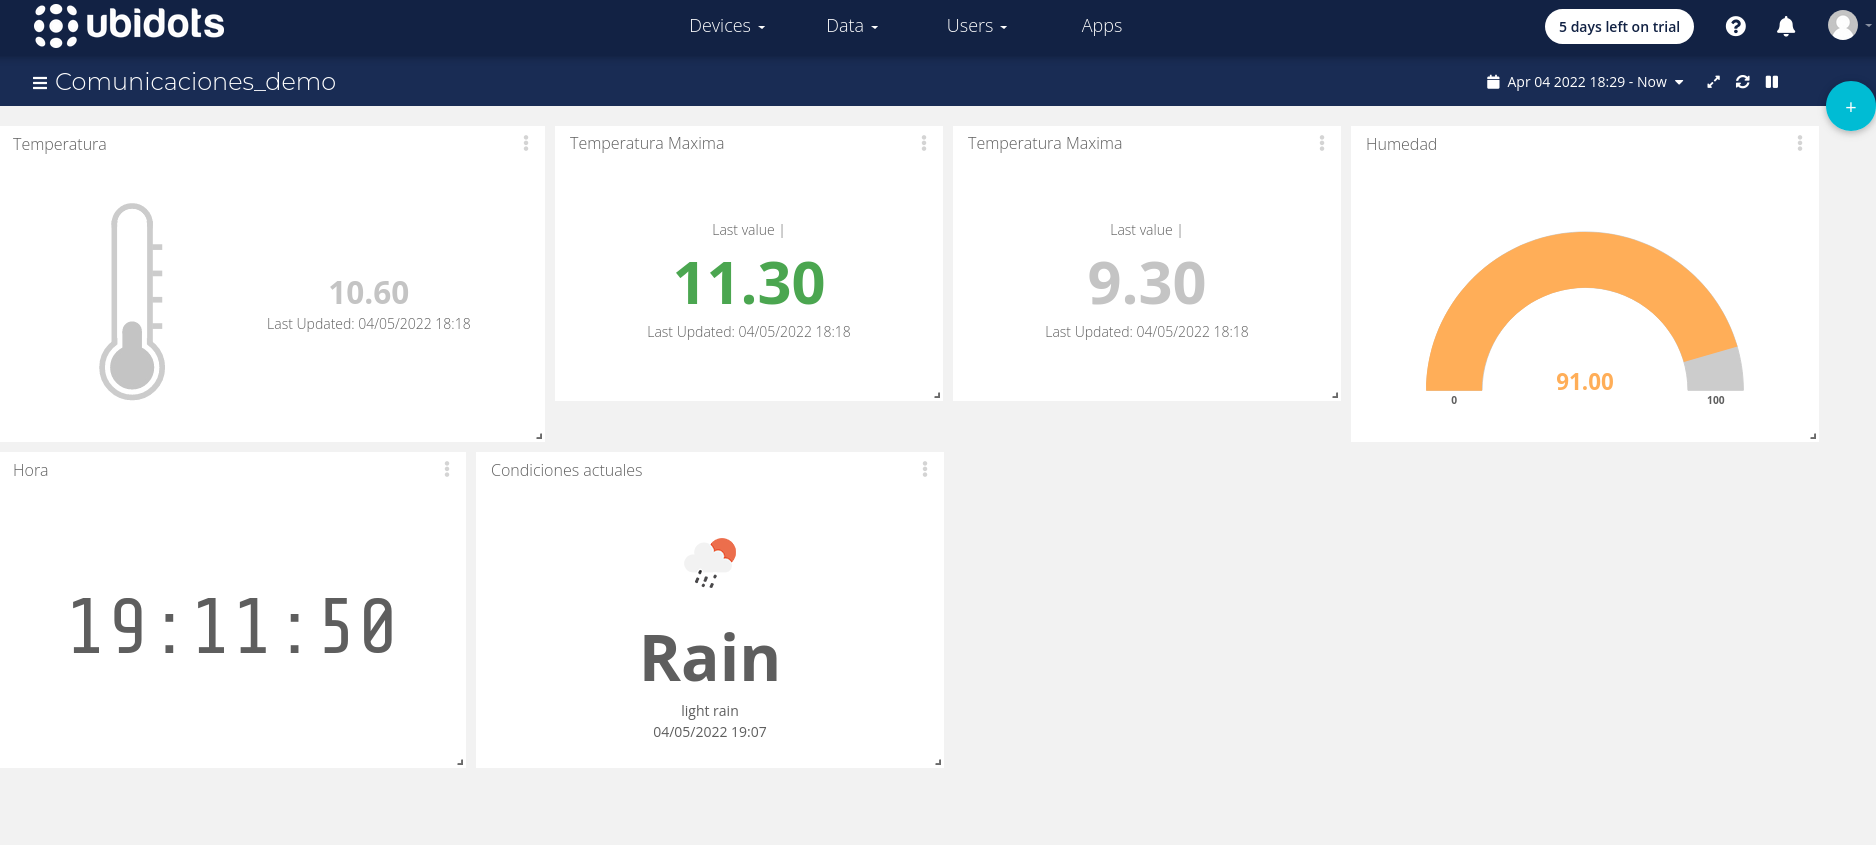
\includegraphics[width=\textwidth]{dashboard_ejemplo.png}
	\caption{Dashboard simple con datos de openweather}
	\label{fig:dashboard_ejemplo}
\end{figure}

Enlace al dashboard creado \url{https://industrial.ubidots.com/app/dashboards/public/dashboard/59mHN0d4o7UrQGhN3BC5KWEvK0hM2c7FXGd-t9ClxBk}

\subsection{Ampliacion de conocimientos}
Se va a realizar una lectura y escritura de datos obtenidos mediante el ESP-32 y la plataforma
ubidots todo el codigo se encuentra adjunto en la practica y en el github para su consulta.
\subsubsection{Enviar valores de del ESP-32 a Ubidots}
Tanto para mandar como para recibir los valores desde el ESP-32 a Ubidots vamos a
utlizar la librería \texttt{UbidotsEsp32Mqtt.h} desde el framework de arduino. El protocolo que utilizamos tanto 
para enviar como recibir los datos es MQTT.


Para mandar los datos a la plataforma Ubidots utlizamos los metodos \texttt{ubidots.add} y \texttt{ubidots.publish}
donde introducimos el nombre del dispositivo y las variables que hemos leido previamente mediante las funciones como puede ser en
nuestro caso \texttt{analogRead()} o \texttt{digitalRead()}.\\

Para saber si la conexion se ha realizado con exito debe aparecer el mensaje de la siguiente figura:

\begin{figure}[h]
	\centering
	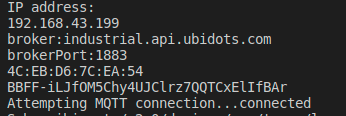
\includegraphics[width=\textwidth]{Mensaje_bienconectado.png}
	\caption{Mensaje debe aparecer en el monitor serie del ESP32}
	\label{fig:mensaje_bien_conectado}
\end{figure}
\pagebreak

Los datos mandados a la Ubidots aparecen de la siguiente forma:
\begin{figure}[h]
	\centering
	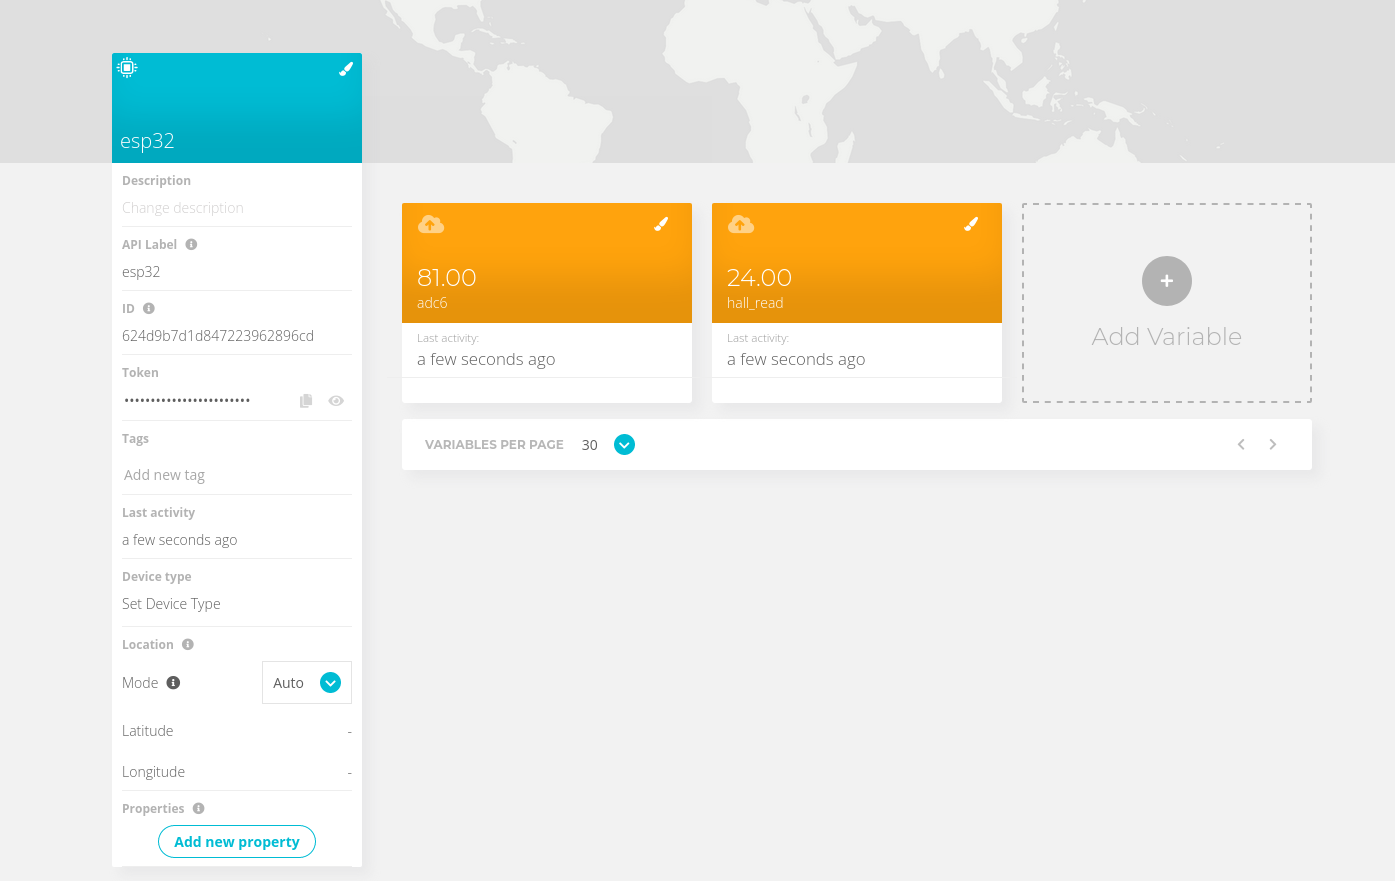
\includegraphics[width=\textwidth]{datos_esp32_ubidots.png}
	\caption{Datos del ADC6 y hall sensor en Ubidots} 
	\label{fig:datos_esp32_ubidots}
\end{figure}
\pagebreak
\begin{figure}[h]
	\centering
	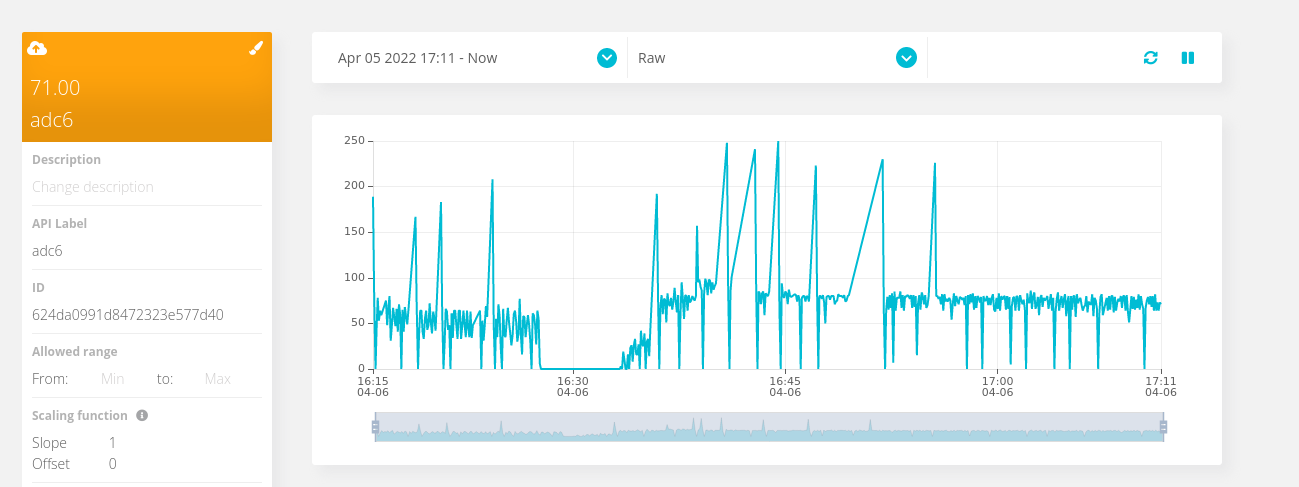
\includegraphics[width=\textwidth]{datos_ADC6.png}
	\caption{Datos proporcionados por el ADC6} 
	\label{fig:datos_esp32_ubidots}
\end{figure}

\subsubsection{Recibir valores de Ubidots a ESP-32}
Para recibir los valores que mandamos a través de node-red a ubidots es un proceso muy similar al de mandar los valores 
en el codigo solamente añadimos la funcion \texttt{ubidots.subscribeLastValue} donde se indica el dispotivo al que nos subscribimos ya la 
variable que queremos leer. Esto no proporciona los valores de la variable por terminal de la siguiente forma:

\begin{figure}[h]
	\centering
	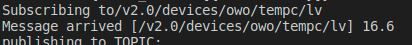
\includegraphics[width=\textwidth]{Temperatura_recibida_ESP32.png}
	\caption{Temperatura leida por el ESP32 a través de Ubidots} 
	\label{fig:temp}
\end{figure}






\section{Bibliografia}

\url{https://help.ubidots.com/en/articles/748067-connect-an-esp32-devkitc-to-ubidots-over-mqtt}\\
\url{https://industrial.ubidots.com}\\
\url{https://www.hackster.io/shahizat005/building-an-esp32-based-iot-weather-station-with-ubidots-05adcc}\\
\end{document}